\documentclass[aspectratio=169,11pt]{beamer}

% --- Theme (portable by default; auto-use metropolis if available) ---
\newif\ifusemetropolis
\IfFileExists{beamerthememetropolis.sty}{\usemetropolistrue}{\usemetropolisfalse}
\ifusemetropolis
  \usetheme[numbering=fraction]{metropolis} % nice minimal look with x/y counter
  \metroset{block=fill,progressbar=foot,sectionpage=progressbar}
\else
  \usetheme{Boadilla}
  \usecolortheme{seahorse}
  \setbeamertemplate{footline}[frame number] % x/y in the footer
\fi
\setbeamertemplate{navigation symbols}{} % hide nav icons

% --- Packages you’ll likely want for math/notation ---
\usepackage{amsmath,amssymb,mathtools}
\usepackage{bm}
\usepackage{graphicx}
\usepackage{booktabs} % tables later if needed
\usepackage{microtype} % nicer text (pdflatex)
\usetikzlibrary{positioning,arrows.meta}

% --- Handy macros for optimization/control ---
\DeclareMathOperator*{\argmin}{arg\,min}
\DeclareMathOperator*{\argmax}{arg\,max}
\newcommand{\R}{\mathbb{R}}
\newcommand{\E}{\mathbb{E}}
\newcommand{\ip}[2]{\left\langle #1,\, #2 \right\rangle}
\newcommand{\norm}[1]{\left\lVert #1 \right\rVert}
\providecommand{\grad}{\nabla}
\providecommand{\hess}{\nabla^2}
\newcommand{\Lag}{\mathcal{L}}

% --- Auto section title frames (useful as your deck grows) ---
\AtBeginSection{
  \begin{frame}[plain]
    \vfill
    \centering
    {\usebeamerfont{title}\insertsection}
    \vfill
  \end{frame}
}

\usetikzlibrary{positioning,arrows.meta}
\tikzset{
  >=Stealth,
  box/.style={
    draw,
    rounded corners,
    align=center,
    inner sep=4pt,
    minimum width=3.2cm,
    minimum height=1.1cm
  }
}


% Use outer theme that shows dots for sections
%\useoutertheme{miniframes}
 



% --- Title info (update these) ---
\title{Lecture 2: Numerical Optimization for Control\\\small(grad/SQP/QP; ALM vs. interior-point vs. penalty)} 
\author{Arnaud Deza}
\institute{ISYE 8803: Special Topics on Optimal Control and Learning}
\date{\today}

 


\begin{document}

% --- Slide 1: Title ---
\begin{frame}[plain]
  \titlepage
\end{frame}
\section{Overview and Big Picture of Lecture 2}

% ---- Learning goals ----
\begin{frame}{Learning goals (what you’ll be able to do)}
\textbf{Goals for today}
\begin{itemize}
\item Pick and configure an optimizer for small control problems (unconstrained \& constrained).
\item Derive KKT conditions and form the SQP/QP subproblems for a nonlinear program.
\item Explain the differences between penalty, augmented Lagrangian, and interior-point methods.
\end{itemize}
\textbf{Why?}\\
In future classes, this will help us map classic control tasks (LQR/MPC/trajectory optimization) to QPs/NLPs and choose a solver strategy.
\end{frame}

% ---- Agenda ----
\begin{frame}{Roadmap for today (2\,hours)}
\begin{enumerate}
\item Big picture and some notation \hfill \textit{(5 min)}
\item Unconstrained optimization: Root-finding, Newton and globalization \hfill \textit{(30 min)}
\item Equality constraints: KKT, Newton vs. Gauss–Newton \hfill \textit{(30 min)}
\item Inequalities \& KKT: complementarity \hfill \textit{(10 min)}
\item Methods: penalty $\rightarrow$ ALM $\rightarrow$ interior-point (PDIP) \hfill \textit{(20 min)}
\item Brief look at SQP for solving hard control problems \hfill \textit{(20 min)} 
\end{enumerate}
\end{frame}



% ---- Big picture ----
\begin{frame}[t]{Big picture: why optimization for control?}
\begin{columns}[T,onlytextwidth]
  \column{0.54\textwidth}
  \small
  \begin{itemize}[<+->]\setlength{\itemsep}{2pt}
    \item Controller synthesis often reduces to solving a sequence of optimization problems.
    \item \textbf{MPC} solves a QP/NLP online at each time step; warm-start and sparsity are critical.
    \item \textbf{Trajectory optimization} (nonlinear robots) uses NLP + collocation; needs robust globalization.
    \item \textbf{Learning-based control} backpropagates through optimizers (differentiable programming).
  \end{itemize}

  \column{0.42\textwidth}
  \centering
  \resizebox{\columnwidth}{!}{%
    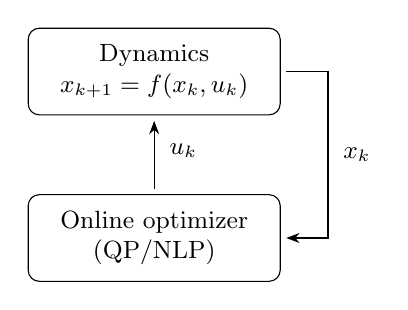
\begin{tikzpicture}[
      node distance=10mm and 12mm,
      every node/.style={font=\small},
      shorten >=2pt,
      shorten <=2pt
    ]
      \node[box] (plant) {Dynamics\\$x_{k+1}=f(x_k,u_k)$};
      \node[box, below=of plant] (opt) {Online optimizer\\(QP/NLP)};

      \draw[->] (opt.north) -- node[pos=0.55, right=2pt] {$u_k$} (plant.south);
      \draw[->] (plant.east) -- ++(0.6,0) |- node[pos=0.25, right=2pt] {$x_k$} (opt.east);
    \end{tikzpicture}%
  }
\end{columns}
\end{frame}

% ===== Slide 1: Derivatives & Jacobians (animated in 4 parts) =====
\begin{frame}{Notation I: derivatives \& Jacobians}

\begin{columns}[T,onlytextwidth]
\column{0.52\textwidth}
\uncover<1->{
\begin{block}{Scalar-valued function}
$f:\mathbb{R}^n \to \mathbb{R}$

\vspace{0.2em}
Row-derivative (row gradient):
\[
\frac{\partial f}{\partial x} \in \mathbb{R}^{1\times n}
\]
\end{block}
}

\uncover<2->{
\begin{block}{First-order model of $f$}
\[
f(x+\Delta x) \approx f(x) + \frac{\partial f}{\partial x}\,\Delta x
\]
\[
\Delta x \in \mathbb{R}^n,\quad \frac{\partial f}{\partial x}\in\mathbb{R}^{1\times n},\quad
\Delta f\in\mathbb{R}
\]
\end{block}
}

\column{0.48\textwidth}
\uncover<3->{
\begin{block}{Vector-valued function}
$g:\mathbb{R}^m \to \mathbb{R}^n$

\vspace{0.2em}
Jacobian:
\[
\frac{\partial g}{\partial y} \in \mathbb{R}^{n\times m}
\]
\end{block}
}

\uncover<4->{
\begin{block}{First-order model of $g$}
\[
g(y+\Delta y) \approx g(y) + \frac{\partial g}{\partial y}\,\Delta y
\]
\[
\Delta y\in\mathbb{R}^m,\quad \frac{\partial g}{\partial y}\in\mathbb{R}^{n\times m},\quad
\Delta g\in\mathbb{R}^n
\]
\end{block}
}
\end{columns}

\end{frame}


% ==== Slide 2 (fits on one page, animated in 4 parts) ====
\begin{frame}{Notation II: gradient, Hessian \& Taylor}
\begingroup
\small
% tighten display math spacing just for this frame
\setlength{\abovedisplayskip}{6pt}
\setlength{\belowdisplayskip}{6pt}
\setlength{\abovedisplayshortskip}{4pt}
\setlength{\belowdisplayshortskip}{4pt}

\begin{columns}[T,onlytextwidth]
  \column{0.48\textwidth}
  \uncover<1->{
  \begin{block}{Gradient (column form)}
  For $f:\mathbb{R}^n\to\mathbb{R}$,
  \[
  \nabla f(x) := \left(\frac{\partial f}{\partial x}\right)^{\!T} \in \mathbb{R}^{n}
  \]
  \end{block}
  }

  \uncover<2->{
  \begin{block}{Hessian}
  \[
  \nabla^2 f(x) := \frac{\partial}{\partial x}\!\left(\frac{\partial f}{\partial x}\right)
  = \frac{\partial^2 f}{\partial x^2} \in \mathbb{R}^{n\times n}
  \]
  \end{block}
  }

  \column{0.52\textwidth}
  \uncover<3->{
  \begin{block}{Shape check}
  \[
  \nabla f(x)\in\mathbb{R}^{n},\quad
  \nabla^2 f(x)\in\mathbb{R}^{n\times n},\quad
  \Delta x\in\mathbb{R}^{n}
  \]
  \[
  \Delta x^{\!T}\nabla^2 f(x)\Delta x \in \mathbb{R}
  \]
  \end{block}
  }

  \uncover<4->{
  \begin{block}{Second-order Taylor}
  \[
  f(x+\Delta x)\approx f(x)
  + \nabla f(x)^{\!T}\Delta x
  + \tfrac{1}{2}\,\Delta x^{\!T}\nabla^2 f(x)\,\Delta x
  \]
  \end{block}
  }
\end{columns}
\endgroup
\end{frame}





\section{Root-Finding}

\begin{frame}{Root Finding}
Given $f(x)$, find $x^*$ such that $f(x^*) = 0$ (example: finding equilibrium of a continuous-time dynamics).

Closely related: fixed point \quad \quad \quad $f(x^*) = x^* \quad (\text{equilibrium of discrete-time dynamics})$

\textbf{Fixed-Point Iteration}
\begin{itemize}
    \item Simplest solution method
    \item If fixed point is stable, just “iterate the dynamics” until it converges
    \item Only works if $x^*$ is a stable equilibrium point and if initial guess is in the basin of attraction
    \item can converge slowly (depends on $f$ i.e depending on eigenvalues)
\end{itemize}
Gradient Descent in Fixed Point Iteration applied to gradient of function $f$.
\end{frame}



\begin{frame}{Newton's Method}
TLDR: Instead os solving for $f(x) =0$, solve a linear for a linear approximation of $f(x)$.\\
Fit a linear approximation to $f(x)$:\quad $f(x+\Delta x) \approx f(x) + \frac{\partial f}{\partial x}\Delta x$

Set approximation to zero and solve for $\Delta x$:

$$
f(x) + \frac{\partial f}{\partial x}\Delta x = 0 \quad \Rightarrow \quad \Delta x = -\left(\frac{\partial f}{\partial x}\right)^{-1} f(x)
$$

Apply correction: $x \leftarrow x + \Delta x$
Do this in a loop and repeat until convergence.

\end{frame}

\begin{frame}{Example: Backward Euler}
Last time: Implicit dynamics model (nonlinear function of current state and future state)
$$
f(x_{n+1}, x_n, u_n) = 0
$$
Implicit Euler: this time we have $x_{n+1}$ on the right; i.e evaluate f at future time.
$$
x_{n+1} = x_n + h f(x_{n+1})
$$

(Evaluate $f$ at future time)

$$
\Rightarrow f(x_{n+1}, x_n, u_n) = x_{n+1} - x_n - h f(x_{n+1}) = 0
$$
Solve root finding problem for $x_{n+1}$
\begin{itemize}
    \item Very fast convergence with Newton (quadratic) and can get machine precision.
    \item Most expensive part is solving a linear system $O(n^3)$
    \item Can improve complexity by taking advantage of problem structure/sparsity.
\end{itemize} 
\end{frame}


\begin{frame}{Move to Julia Code}
\begin{center}
    \textbf{Quick Demo of Julia Notebook: part1\_root\_finding.ipynb}
\end{center}
\end{frame}


\begin{frame}{Minimization}
$$
\min_x f(x), \quad f(x): \mathbb{R}^n \to \mathbb{R}
$$
If $f$ is smooth, $\frac{\partial f}{\partial x}(x^*) = 0$ at a local minimum. 

Hence, now we have a root-finding problem $\nabla f(x) = 0$ $\Rightarrow$ Apply Newton!

$$
\nabla f(x+\Delta x) \approx \nabla f(x) + \frac{\partial}{\partial x}(\nabla f(x))\Delta x = 0
\quad \quad \quad \quad 
\Rightarrow \Delta x = -(\nabla^2 f(x))^{-1}\nabla f(x)
$$

$$
x \leftarrow x + \Delta x
$$

Repeat this step until convergence; Intuition to have about Newton:
\begin{itemize}
    \item Fitting a quadratic approximation to $f(x)$; Exactly minimize approximation
\end{itemize} 
    
\end{frame}


\begin{frame}{Move to Julia Code}
\begin{center}
    \textbf{Quick Demo of Julia Notebook: part1\_minimization.ipynb}
\end{center}
\end{frame}



\begin{frame}{Take-away Messages on Newton}
Newton is a local root-finding method. Will converge to the closest fixed point to the initial guess (min, max, saddle). 

\textbf{Sufficient Conditions}
\begin{itemize}
    \item $\nabla f = 0$: “first-order necessary condition” for a minimum. Not a sufficient condition.
    \item  Let’s look at scalar case: $\Delta x = -\frac{1}{\nabla^2 f}\nabla f$
\end{itemize} 
where: negative corresponds to “descent”, $\nabla f$ corresponds to the gradient and $\nabla^2 f$ acts as the “leading rate” / “step size”.

$\nabla^2 f > 0 \quad \Rightarrow \quad \text{descent (minimization)} \quad \quad \quad \nabla^2 f < 0 \quad \Rightarrow \quad \text{ascent (maximization)}$
\begin{itemize}
    \item In $\mathbb{R}^n$, if $\nabla^2 f \succeq 0$ (positive definite) $\Rightarrow$ descent
    \item If $\nabla^2 f > 0$ everywhere $\Rightarrow f(x)$ is strongly convex → Can always solve with Newton
    \item Usually not the case for hard/nonlinear problems
\end{itemize}
 \end{frame}

\begin{frame}{Regularization: Ensuring Local Minimization}
Practical solution to make sure we always minimize:
 
If $H$ ($H \leftarrow \nabla^2 f$) not positive definite, we just make it so with regularization.


While $H \not\succeq 0$:
$$H \leftarrow H + \beta I \quad (\beta > 0 \ \text{scalar hyperparameter})$$
 
Then do newton step as usual. I.e:

$$
x \quad \leftarrow \quad  x + \Delta x \quad  = \quad x  -H^{-1}\nabla f
$$

\begin{itemize}
    \item also called “damped Newton” (shrinks steps)
    \item Guarantees descent
    \item Regularization makes sure we minimize, but what about over-shooting?
\end{itemize} 
\end{frame}

\begin{frame}{Line Search: Mitigating overshooting in Newton}
\begin{itemize}
    \item Often $\Delta x$ step from Newton overshoots the minimum.
    \item To fix this, check $f(x + \alpha \Delta x)$ and “back track” until we get a “good” reduction.
    \item Many strategies: all differ in definition of good. 
    \item A simple + effective one is \textbf{Armijo Rule}:
\end{itemize} 

Start with $\alpha=1$ as our step length and have tolerance $b$ as a hyper-parameter.
 $$
\text{while } f(x + \alpha \Delta x) > f(x) + b \alpha \nabla f(x)^T \Delta x: \quad \quad  \alpha \leftarrow c \alpha \quad (\text{scalar } < 1 \text{ i.e } c =\frac{1}{2}) 
$$ 
\footnotesize
The intuition behind this is that $\alpha \nabla f(x)^T \Delta x$ corresponds to the expected change in $f$ based on a 1st order taylor series expansion. I.e we are checking the actual decrease in $f$ agrees with a $1st$ order taylor approximation within a tolerance $b$.
    
\end{frame} 

%\section{Part II -- Equality constraints: KKT, Newton vs. Gauss–Newton}
\section{Constrained Optimization}

% ==== Equality constraints: KKT, Newton vs. Gauss–Newton ====

\begin{frame}{Equality-constrained minimization: geometry and conditions}
\textbf{Problem}; $\min_{x\in\mathbb{R}^n} f(x)\quad \text{s.t.}\quad C(x)=0, C:\mathbb{R}^n\to\mathbb{R}^m$.

\medskip
\textbf{Geometric picture.} At an optimum on the manifold $C(x)=0$, the negative gradient must lie in the tangent space:

$$
\grad f(x^\star)\ \perp\ \mathcal{T}_{x^\star}=\{p:\; J_C(x^\star)p=0\}.
$$

Equivalently, the gradient is a linear combination of constraint normals:

$$
\grad f(x^\star)+J_C(x^\star)^{\!T}\lambda^\star=0,\qquad C(x^\star)=0\quad(\lambda^\star\in\mathbb{R}^m).
$$

\medskip
\textbf{Lagrangian.}; $L(x,\lambda)=f(x)+\lambda^{\!T}C(x)$.
\end{frame}

\begin{frame}{A nicer visual explanation/derivation of KKT conditions}
\begin{center}
    Quick little whiteboard derivation
\end{center}
    
\end{frame}



\section{Constrained Optimization}

% ==== Slide 1: Picture-first intuition ====
\begin{frame}[t]{Equality constraints: picture first}
\setbeamercovered{invisible}

\textbf{Goal.} Minimize $f(x)$ while staying on the surface $C(x)=0$.

\uncover<2->{\textbf{Feasible set as a surface.} Think of $C(x)=0$ as a smooth surface embedded in $\mathbb{R}^n$ (a manifold).}
 
\uncover<3->{\textbf{Move without breaking the constraint.} Tangent directions are the “along-the-surface” moves that keep $C(x)$ unchanged to first order. Intuitively: tiny steps that slide on the surface.}
 
\uncover<4->{\textbf{What must be true at the best point.} At $x^\star$, there is no downhill direction that stays on the surface. Equivalently, the usual gradient of $f$ has \emph{no component along the surface}.}
 
\uncover<5->{\textbf{Normals enter the story.} If the gradient can’t point along the surface, it must point \emph{through} it—i.e., it aligns with a combination of the surface’s normal directions (one normal per constraint).}
\end{frame}

% ==== Slide 2: From picture to KKT ====
\begin{frame}[t]{From the picture to KKT (equality case)}
\setbeamercovered{invisible}

\textbf{KKT conditions at a regular local minimum (equality only):}
 
\uncover<1->{\textbf{1) Feasibility:} $C(x^\star)=0$. \emph{(We’re on the surface.)}}
 
\uncover<2->{\textbf{2) Stationarity:} $\nabla f(x^\star) + J_C(x^\star)^{\!T}\lambda^\star = 0$. \emph{(The gradient is a linear combination of the constraint normals.)}}
 
\uncover<3->{\textbf{Lagrangian viewpoint.} Define $L(x,\lambda)=f(x)+\lambda^{\!T}C(x)$. At a solution, $x^\star$ is a stationary point of $L$ w.r.t.\ $x$ (that’s the stationarity equation), while $C(x^\star)=0$ enforces feasibility.}
 
\uncover<4->{\textbf{What the multipliers mean.} The vector $\lambda^\star$ tells how strongly each constraint “pushes back” at the optimum; it also measures sensitivity of the optimal value to small changes in the constraints.}
 
\end{frame}


\begin{frame}{KKT system for equalities (first-order necessary conditions)}
\textbf{KKT (FOC).}

$$
\grad_x L(x,\lambda)=\grad f(x)+J_C(x)^{\!T}\lambda=0,\qquad \grad_\lambda L(x,\lambda)=C(x)=0.
$$

\textbf{Solve by Newton on KKT:} linearize both optimality and feasibility:

$$
\begin{bmatrix}
\hess f(x) + \sum_{i=1}^m \lambda_i\,\hess C_i(x) & J_C(x)^{\!T}\\[2pt]
J_C(x) & 0
\end{bmatrix}
\begin{bmatrix}\Delta x\\ \Delta\lambda\end{bmatrix}
=-
\begin{bmatrix}
\grad f(x)+J_C(x)^{\!T}\lambda\\ C(x)
\end{bmatrix}.
$$

\textit{Notes.} This is a symmetric \emph{saddle-point} system; typical solves use block elimination (Schur complement) or sparse factorizations.
\end{frame}






\begin{frame}{Move to Julia Code}
\begin{center}
    \textbf{Quick Demo of Julia Notebook: part2\_eq\_constraints.ipynb}
\end{center}
\end{frame}

\begin{frame}{Numerical practice: Newton on KKT}
  \setbeamercovered{invisible}

  
    \textbf{When it works best.}
    \begin{itemize}
      \item Near a regular solution with $J_{C}(x^\star)$ full row rank and positive-definite reduced Hessian.
      \item With a globalization (line search on a merit function) and mild regularization for robustness.
    \end{itemize}

    % --- Part 2: appears on the 2nd click only --- 
    \uncover<2->{%
      \textbf{Common safeguards.}
      \begin{itemize}
        \item \emph{Regularize} the $(1,1)$ block to ensure a good search direction (e.g., add $\beta I$).
        \item \emph{Merit/penalty} line search to balance feasibility vs.\ optimality during updates.
        \item \emph{Scaling} constraints to improve conditioning of the KKT system.
      \end{itemize}
    } 
\end{frame}


\begin{frame}{Gauss--Newton vs. full Newton on KKT}

\uncover<1->{
\textbf{Full Newton Hessian of the Lagrangian:}\quad
$\nabla_{xx}^2 L(x,\lambda) = \nabla^2 f(x) + \sum_{i=1}^m \lambda_i\, \nabla^2 C_i(x)$
}

\vspace{0.6em}

\uncover<2->{
\textbf{Gauss--Newton approximation:} drop the \emph{constraint-curvature} term
$\sum_{i=1}^m \lambda_i\, \nabla^2 C_i(x)$:
\begin{align*}
H_{\text{GN}}(x) &\approx \nabla^2 f(x).
\end{align*}
}

\uncover<3->{
\textbf{Trade-offs (high level).}
\begin{itemize}
  \item \emph{Full Newton:} fewer iterations near the solution, but each step is costlier and can be less robust far from it.
  \item \emph{Gauss--Newton:} cheaper per step and often more stable; may need more iterations but wins in wall-clock on many problems.
\end{itemize}
}

\end{frame}


% ==== Inequalities & KKT: complementarity ====

\begin{frame}{Inequality-constrained minimization and KKT}
\textbf{Problem.} $\quad \quad \min f(x)\quad\text{s.t.}\quad c(x)\ge 0,  \quad \quad c:\mathbb{R}^n\to\mathbb{R}^p$.

\textbf{KKT conditions (first-order).}

$$
\begin{aligned}
&\text{Stationarity:} && \grad f(x)-J_c(x)^{\!T}\lambda=0,\\
&\text{Primal feasibility:} && c(x)\ge 0,\\
&\text{Dual feasibility:} && \lambda\ge 0,\\
&\text{Complementarity:} && \lambda^{\!T}c(x)=0\quad(\text{i.e., }\lambda_i c_i(x)=0\ \forall i).
\end{aligned}
$$

\textbf{Interpretation.}
\begin{itemize}
\item \emph{Active} constraints: $c_i(x)=0 \Rightarrow \lambda_i\ge 0$ can be nonzero (acts like an equality).
\item \emph{Inactive} constraints: $c_i(x)>0 \Rightarrow \lambda_i=0$ (no influence on optimality).
\end{itemize}
\end{frame}




\begin{frame}{Complementarity in plain English (and why Newton is tricky)}
\footnotesize

\textbf{What $\lambda_i c_i(x)=0$ means.}
\begin{itemize}
\item Tight constraint ($c_i=0$) $\Rightarrow$ can press back ($\lambda_i\ge0$).
\item Loose constraint ($c_i>0$) $\Rightarrow$ no force ($\lambda_i=0$).
\end{itemize}

\textbf{Why naive Newton fails.}
\begin{itemize}
\item Complementarity = nonsmooth + inequalities ($\lambda\ge0$, $c(x)\ge0$).
\item Equality-style Newton can violate nonnegativity or bounce across boundary.
\end{itemize}

\textbf{Two main strategies (preview).}
\begin{itemize}
\item \emph{Active-set:} guess actives $\Rightarrow$ solve equality-constrained subproblem, update set.
\item \emph{Barrier/PDIP/ALM:} smooth or relax complementarity, damped Newton, drive relaxation $\to 0$.
\end{itemize}
\end{frame}



 
\section{Minimization w/ Inequality Constraints}

\begin{frame}{Three families you should know (high level)}
\textbf{Goal:} Handle inequalities $c(x)\ge 0$ (and equalities) robustly and efficiently.

\medskip
\textbf{Families.}
\begin{enumerate}
\item \textbf{Penalty}: embed violations in the objective; crank a parameter $\rho\uparrow$.
\item \textbf{Augmented Lagrangian (ALM)}: maintain multipliers \& a \emph{moderate} penalty; solve easier subproblems.
\item \textbf{Interior-Point (PDIP)}: enforce $c(x)>0$ via a barrier; follow the \emph{central path} with primal--dual Newton.
\end{enumerate}

\textbf{Rule of thumb.} Penalty is simplest; ALM is a strong default for medium accuracy; PDIP is the gold standard for convex QPs and very robust with Newton. 
\end{frame}




\begin{frame}{Inequality-Constrained Minimization}
\textbf{Problem Setup:}
$$
\min f(x) \quad \text{s.t. } c(x) \geq 0
$$
\textbf{KKT conditions:} 

$$
\nabla f - \left(\frac{\partial c(x)}{\partial x}\right)^T \lambda = 0 \quad \text{(stationarity)}
$$

$$
c(x) \geq 0 \quad \text{(primal feasibility)} \quad \quad \quad  \lambda \geq 0 \quad \text{(dual feasibility)}
$$ 

$$
\lambda \circ c(x) = \lambda^T c(x) = 0 \quad \text{(complementarity)}
$$

\textbf{Unlike equality case, we can’t directly solve KKT conditions with Newton! Why?}

 
\end{frame}


\begin{frame}{Lots of solution methods to use: Active Set Method} 
\underline{\textbf{Active Set Method}}
\begin{itemize}
    \item High level idea: Guess which inequalities are redundant at optimality and throw them away.
    \item Switch inequality constraints on/off in outer-loop and solve equality-constrained problem.
    \item Works well if you can guess active set well ( common in MPC where good warm-starts are common).
    \item Has really bad worst-time complexity.
    \item Usually custom heuristics are used for specific problem classes/structure.

\end{itemize}
\end{frame}

% --- Slide 1: Idea & Algorithm ---------------------------------------------
\begin{frame}{Penalty Methods: Idea \& Algorithm}
\underline{\textbf{Penalty Method}}: Replace constraints with cost terms that penalize violation!
\[
\min_x\; f(x) \;+\; \tfrac{\rho}{2}\,\big\|c^-(x)\big\|_2^2,\qquad
c^-(x):=\min(0,c(x))\ \text{(elementwise)}.
\]

\textbf{Algorithm sketch.}
\begin{enumerate}
\item Start with a small $\rho>0$; minimize the penalized unconstrained objective.
\item Increase $\rho$ (e.g., $\times 10$) and warm start from previous $x$.
\item Stop when $c^-(x)$ is small enough.
\end{enumerate}
\end{frame}


% --- Slide 3: Quadratic penalty & why large $\rho$ is needed ----------------
\begin{frame}{Quadratic penalty: need large $\rho$ for strong feasibility pressure}
\begin{columns}[T,onlytextwidth]
\column{0.45\textwidth}
\small
\textbf{Pros.} Dead simple; reuse unconstrained machinery (Grad/Newton + line search). \\
\textbf{Cons.} Ill-conditioning as $\rho\to\infty$; struggles to reach high accuracy; multipliers are implicit. \\
\textbf{Popular fix.} Estimate $\lambda$ (Augmented Lagrangian / ADMM) to converge with finite $\rho$.

\vspace{0.6em}
\textbf{Takeaway.} The penalty outside the feasible set ($x<0$ here) is only quadratic,
so to make violations tiny you often must crank $\rho$ very large $\Rightarrow$ poor conditioning.

\column{0.53\textwidth}
\centering
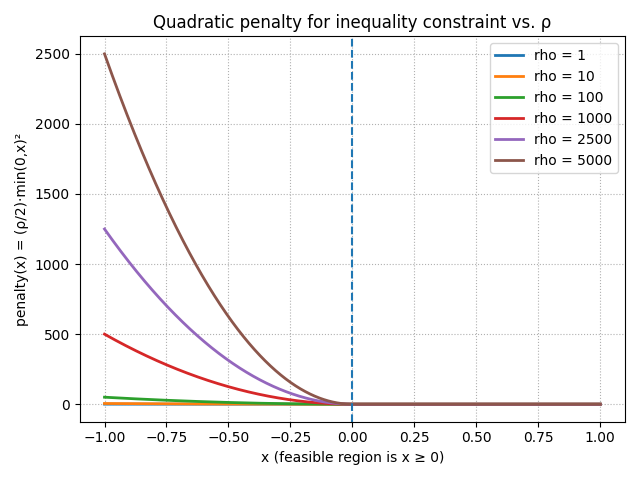
\includegraphics[width=\textwidth]{figures/quadratic_penalty.png}
\end{columns}
\end{frame}







% ---- ALM ---- 
\begin{frame}[t]{Augmented Lagrangian (ALM): fix penalty’s weaknesses}
\setbeamercovered{invisible}

\uncover<1->{\textbf{Core idea.}\; Introduce multipliers $\lambda$ so we can keep $\rho$ moderate and still achieve accuracy.}
 
\uncover<2->{\textbf{Lagrangian for equality case:}\;
$\displaystyle \mathcal{L}_\rho(x,\lambda)=f(x)+\lambda^{\!T}C(x)+\tfrac{\rho}{2}\|C(x)\|_2^2.$}
 
\uncover<3->{\textbf{Outer loop.}
\begin{enumerate}
  \item $x^{k+1}\approx \arg\min_x \mathcal{L}_\rho(x,\lambda^k)$ (unconstrained solve).
  \item $\lambda^{k+1}=\lambda^k+\rho\,C(x^{k+1})$.
\end{enumerate}
}
 
\uncover<4->{\textbf{Inequalities (sketch).}\; Apply to the \emph{hinge} $c^-(x)$ and keep $\lambda\ge 0$:
\[
\mathcal{L}_\rho(x,\lambda)=f(x)-\lambda^{\!T}c(x)+\tfrac{\rho}{2}\|c^-(x)\|_2^2,\quad
\lambda^{k+1}=\max\!\big(0,\lambda^k-\rho\,c(x^{k+1})\big).
\]
}

\uncover<5->{\textbf{Why it works.}\; Subproblems are better conditioned than pure penalty; $\lambda$ estimates improve the model; finite $\rho$ can reach high accuracy.}
\end{frame}




\begin{frame}{ALM in practice (optimization loop view)}
\textbf{Inner solver.} Use (damped) Newton or quasi-Newton on $\mathcal{L}_\rho(\cdot,\lambda^k)$ with Armijo/Wolfe line search. \\
\textbf{Tuning.}
\begin{itemize}
\item Keep $\rho$ fixed or adapt slowly (increase if feasibility stalls).
\item Scale constraints; monitor $|C(x)|$ and stationarity.
\end{itemize}
\textbf{When to pick ALM.}
\begin{itemize}
\item Nonconvex NLPs where feasibility progress matters and you want robust globalization.
\item When medium accuracy is tolerable/fine, or as a precursor to a polished PDIP phase on a convex QP.
\end{itemize}

\end{frame}









\begin{frame}{Interior-Point / Barrier Methods}
\underline{\textbf{TLDR: }} Replace inequalities with barrier function in objective:

$$
\min f(x), \quad x \geq 0 \quad \to \quad \min f(x) - \rho \log(x)
$$

\begin{itemize} 
    \item Gold standard for convex problems.
    \item Fast convergence with Newton and strong theoretical properties.
    \item Used in IPOPT.
\end{itemize} 
\end{frame}


% --- Slide 2: Barrier intuition (contrast) ---------------------------------
\begin{frame}{Barrier intuition issue: $-\log(x)$ blows up near the boundary}
\centering
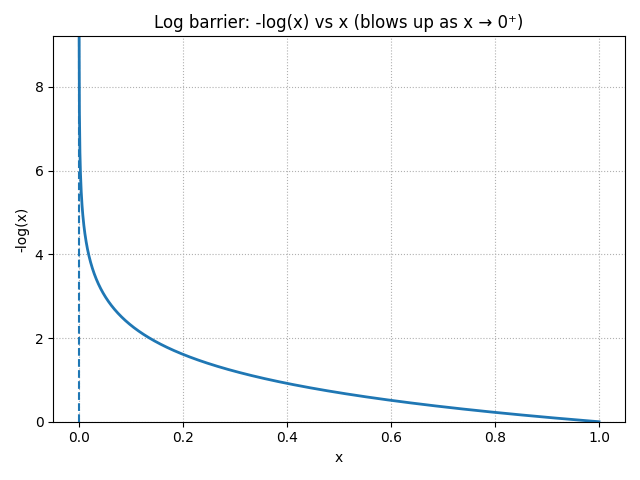
\includegraphics[scale=0.5]{figures/log_barrier.png}
 
{\small
For an inequality like $x\ge 0$, the log barrier $-\log(x)$ goes to $\infty$ as $x\to 0^+$,
creating a \emph{hard wall} at the boundary (contrast with quadratic penalties).
}
\end{frame}



\begin{frame}{Primal-Dual Interior Point Method}
$$
\min f(x) \quad \text{s.t. } x \geq 0
$$

$$
\to \min f(x) - \rho \log(x)
$$

$$
\frac{\partial f}{\partial x} - \frac{\rho}{x} = 0
$$

\begin{itemize}
    \item This “primal” FON condition blows up as $x \to 0$.
    \item We can fix this with the “primal-dual trick.”
\end{itemize}
\end{frame}  


\begin{frame}{The Primal-Dual Trick for IPM}
Introduce new variable $\lambda = \frac{\rho}{x} \quad \Rightarrow \quad x \lambda = \rho$.

$$
\begin{cases}
\nabla f - \lambda = 0 \\
x \lambda = \rho
\end{cases}
$$


\begin{itemize}
    \item This can actually be viewed as a relaxed complementarity slackness from KKT!
    \item Converges to exact KKT solution as $\rho \to 0$.
    \item We lower $\rho$ gradually as solver converges (from $\rho \sim 1$ to $\rho \sim 10^{-6}$).
    \item Note: we still need to enforce $x \geq 0$ and $\lambda \geq 0$ (with line search).
\end{itemize} 
\textbf{We will use another approach from 2022 from a researcher at TRI that developped an even cooler trick.}
    
\end{frame}

\begin{frame}{Log-Domain Interior-Point Method}
\begin{center}
    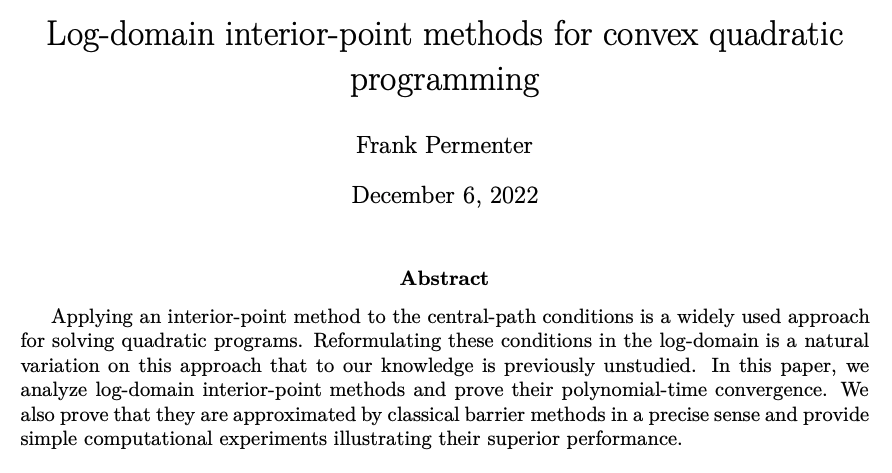
\includegraphics[scale=0.4]{figures/tri_paper.png}
\end{center}
\end{frame}


\begin{frame}{Log-Domain Interior-Point Method}
\textbf{More general constraint case}:   \quad \quad \quad \quad \quad  $\min f(x) \quad \text{s.t. } c(x) \geq 0$

\textbf{Simplify by introducing a “slack variable”:}

$$
\min_{x,s} f(x) \quad \text{s.t. } c(x) - s = 0, \; s \geq 0
$$

$$
\to \min_{x,s} f(x) - \rho \log(s)  \quad \text{s.t. } c(x) - s = 0
$$

\textbf{ Write out Lagrangian:} \quad \quad \quad $L(x,s,\lambda) = f(x) - \rho \log(s) - \lambda^T(c(x)-s)$  
\end{frame}


\begin{frame}{Log-Domain Interior-Point Method}
\textbf{Apply F.O.N.C to Lagrangian from last slide:}

$$
\nabla_x L = \nabla f - \left(\frac{\partial c}{\partial x}\right)^T \lambda = 0
$$

$$
\nabla_s L = \frac{\rho}{s} + \lambda = 0 \quad \Rightarrow \quad s \lambda = \rho
$$

$$
\nabla_\lambda L = s - c(x) = 0
$$

This second equation has a really nice interpretation: relaxed complementarity slackness


\end{frame}





\begin{frame}{Log-Domain Interior-Point Method}

\textbf{Change of variables (elementwise):}
\[
\boxed{\ \rho := s \circ \lambda,\qquad 
\sigma := \tfrac{1}{2}\big(\log s - \log \lambda\big)\ }
\quad\Longleftrightarrow\quad
\boxed{\ s = \sqrt{\rho}\, \circ e^{\sigma},\quad 
\lambda = \sqrt{\rho}\, \circ e^{-\sigma}\ }
\]
{\footnotesize
Here \(\circ\) is the Hadamard (elementwise) product; \(s,\lambda,\rho,\sigma\in\mathbb{R}^m\) with \(s>0,\lambda>0\).
By construction \(s\ge 0,\ \lambda\ge 0\) and \(\rho = s\circ\lambda\) (the relaxed complementarity) holds.}

\vspace{0.6em}

\textbf{KKT (first-order) residuals with inequality \(c(x) - s = 0\):}
\[
r_x(x,\sigma) := \nabla f(x) - J(x)^{\!T}\lambda(\sigma), 
\qquad
r_c(x,\sigma) := c(x) - s(\sigma) = 0,
\]
where \(J(x) := \frac{\partial c}{\partial x}(x)\), 
\(s(\sigma)=\sqrt{\rho}\circ e^{\sigma}\), 
\(\lambda(\sigma)=\sqrt{\rho}\circ e^{-\sigma}\).

\end{frame}

\begin{frame}{Log-Domain Interior-Point Method}

\textbf{(Gauss-)Newton step in \((x,\sigma)\) for fixed \(\rho\):}
\[
\begin{bmatrix}
H & J^{\!T}\Lambda \\[2pt]
J & -S
\end{bmatrix}
\begin{bmatrix}
\delta x \\ \delta \sigma
\end{bmatrix}
=
-
\begin{bmatrix}
r_x \\ r_c
\end{bmatrix}
\quad\text{with}\quad
S:=\operatorname{diag}(s),\ \Lambda:=\operatorname{diag}(\lambda).
\]
{\footnotesize
Here \(H\) is your Hessian model w.r.t.\ \(x\):
\(
H=\nabla^2 f(x)\ \) (Gauss--Newton/curvature-drop), 
or 
\(
H=\nabla^2 f(x)-\sum_{i=1}^m \lambda_i \nabla^2 c_i(x)
\) (full Newton). 
Note the simple sensitivities:
\(ds = S\,d\sigma,\ d\lambda = -\Lambda\,d\sigma\), 
which produce the block entries \(-S\) and \(J^{\!T}\Lambda\).
}

\end{frame}




\begin{frame}{Log-Domain Interior-Point Method (easier notation)}
\textbf{To ensure $s \geq 0$ and $\lambda \geq 0$, introduce change of variables:} $$s = \sqrt{\rho} e^{\sigma}, \quad \lambda = \sqrt{\rho} e^{-\sigma}$$

Now (relaxed) complementarity is \textbf{always satisfied} by construction!

Plug back into F.O.N.C

$$
\nabla f - \left(\frac{\partial c}{\partial x}\right)^T \lambda = 0 \quad \quad \quad c(x) - \sqrt{\rho} e^{\sigma} = 0
$$

We can solve these with (Gauss) Newton:

$$
\begin{bmatrix}
H & \sqrt{\rho} c^T e^{-\sigma} \\
c & -\sqrt{\rho} e^{\sigma}
\end{bmatrix}
\begin{bmatrix}
\delta x \\ \delta \sigma
\end{bmatrix}
=
\begin{bmatrix}
-\nabla f + c^T \lambda \\ -c(x) + \sqrt{\rho} e^{\sigma}
\end{bmatrix}
$$



\end{frame}






\begin{frame}{Example: Quadratic Program}
Super common problem to be solved in control applications: quadratic programs
$$
\min_x \tfrac{1}{2} x^T Q x + q^T x, \quad Q \succeq 0
$$

s.t.

$$
Ax = b, \quad Cx \leq d
$$

\begin{itemize}
    \item Super useful in control (SQP)
    \item Can be solved very fast ($\sim kHz$).
\end{itemize} 
\end{frame}



\begin{frame}{Move to Julia Code}
\begin{center}
    \textbf{Quick Demo of Julia Notebook: part3\_ipm.ipynb}
\end{center}
\end{frame}


% ---- Comparison (animated main bullets) ----
\begin{frame}{Penalty vs.\ ALM vs.\ PDIP: what changes?}
\begin{itemize}
  \item<1-> \textbf{Feasibility handling:}
    \begin{itemize}
      \item Penalty: encourages $c(x)\ge 0$ via cost; feasibility only in the limit $\rho\uparrow$.
      \item ALM: balances optimality and feasibility via $\lambda$ updates at finite $\rho$.
      \item PDIP: enforces strict interior $c(x)>0$; drives $s_i\lambda_i=\rho\to 0$.
    \end{itemize}

  \item<2-> \textbf{Conditioning:}
    \begin{itemize}
      \item Penalty gets ill-conditioned as $\rho$ grows.
      \item ALM keeps conditioning reasonable.
      \item PDIP maintains well-scaled Newton systems near the path (with proper scaling).
    \end{itemize}

  \item<3-> \textbf{Accuracy:} Penalty (low–med), ALM (high with finite $\rho$), PDIP (high; excellent for convex).

  \item<4-> \textbf{Per-iteration work:} Penalty/ALM solve unconstrained-like subproblems; PDIP solves structured KKT systems with slacks/duals.
\end{itemize}
\end{frame}

 
\section{Sequential Quadratic Programming (SQP)}

% ------------------------------------------------
\begin{frame}{What is SQP?}
\textbf{Idea:} Solve a nonlinear, constrained problem by repeatedly solving a \emph{quadratic program (QP)} built from local models.\\[4pt]
\begin{itemize}
  \item Linearize constraints; quadratic model of the Lagrangian/objective.
  \item Each iteration: solve a QP to get a step \(d\), update \(x \leftarrow x + \alpha d\).
  \item Strength: strong local convergence (often superlinear) with good Hessian info.
\end{itemize}
\end{frame}

% ------------------------------------------------
\begin{frame}{Target Problem (NLP)}
\[
\min_{x \in \R^n} \ f(x)
\quad
\text{s.t.}\quad
g(x)=0,\quad h(x)\le 0
\]
\begin{itemize}
  \item \(f:\R^n\!\to\!\R\), \(g:\R^n\!\to\!\R^{m}\) (equalities), \(h:\R^n\!\to\!\R^{p}\) (inequalities).
  \item KKT recap (at candidate optimum \(x^\star\)): 
\[
\exists \ \lambda \in \R^{m},\ \mu \in \R^{p}_{\ge 0}:
\ \grad f(x^\star) + \nabla g(x^\star)^T\lambda + \nabla h(x^\star)^T \mu = 0,
\]
\[
g(x^\star)=0,\quad h(x^\star)\le 0,\quad \mu \ge 0,\quad \mu \odot h(x^\star) = 0.
\]
\end{itemize}
\end{frame}

% ------------------------------------------------
\begin{frame}{From NLP to a QP (Local Model)}
At iterate \(x_k\) with multipliers \((\lambda_k,\mu_k)\):\\[4pt]
\textbf{Quadratic model of the Lagrangian}
\[
m_k(d) = \ip{\grad f(x_k)}{d} + \tfrac{1}{2} d^T B_k d
\]
with \(B_k \approx \nabla^2_{xx}\Lag(x_k,\lambda_k,\mu_k)\).\\[6pt]
\textbf{Linearized constraints}
\[
g(x_k) + \nabla g(x_k)\, d = 0,\qquad
h(x_k) + \nabla h(x_k)\, d \le 0.
\]
\end{frame}

% ------------------------------------------------
\begin{frame}{The SQP Subproblem (QP)}
\[
\begin{aligned}
\min_{d \in \R^n}\quad & \grad f(x_k)^T d + \tfrac{1}{2} d^T B_k d \\
\text{s.t.}\quad & \nabla g(x_k)\, d + g(x_k) = 0, \\
& \nabla h(x_k)\, d + h(x_k) \le 0.
\end{aligned}
\]
\begin{itemize}
  \item Solve QP \(\Rightarrow\) step \(d_k\) and updated multipliers \((\lambda_{k+1},\mu_{k+1})\).
  \item Update \(x_{k+1} = x_k + \alpha_k d_k\) (line search or trust-region).
\end{itemize}
\end{frame}

% ------------------------------------------------
\begin{frame}{Algorithm Sketch (SQP)}
\begin{enumerate}
  \item Start with \(x_0\), multipliers \((\lambda_0,\mu_0)\), and \(B_0 \succ 0\).
  \item Build QP at \(x_k\) with \(B_k\), linearized constraints.
  \item Solve QP \(\Rightarrow\) get \(d_k\), \((\lambda_{k+1},\mu_{k+1})\).
  \item Globalize: line search on merit or use filter/TR to choose \(\alpha_k\).
  \item Update \(x_{k+1} = x_k + \alpha_k d_k\), update \(B_{k+1}\) (e.g., BFGS).
\end{enumerate}
\end{frame}

% ------------------------------------------------
\begin{frame}{Toy Example (Local Models)}
\textbf{Problem:}
\[
\min_{x\in\R^2} \ \tfrac{1}{2}\norm{x}^2
\quad \text{s.t.} \quad g(x)=x_1^2 + x_2 - 1 = 0,\ \ h(x)=x_2 - 0.2 \le 0.
\]
At \(x_k\), build QP with
\[
\grad f(x_k)=x_k,\quad B_k=I,\quad
\nabla g(x_k) = \begin{bmatrix} 2x_{k,1} & 1 \end{bmatrix},\ 
\nabla h(x_k) = \begin{bmatrix} 0 & 1 \end{bmatrix}.
\]
Solve for \(d_k\), then \(x_{k+1}=x_k+\alpha_k d_k\).
\end{frame}
 

% ------------------------------------------------
\begin{frame}{Globalization: Making SQP Robust}
SQP is an important method, and there are many issues to be considered to obtain an \textbf{efficient} and \textbf{reliable} implementation:
\begin{itemize}
  \item Efficient solution of the linear systems at each Newton Iteration (Matrix block structure can be exploited.
  \item Quasi-Newton approximations to the Hessian.
  \item Trust region, line search, etc. to improve robustnes (i.e TR: restrict \(\norm{d}\) to maintain model validity.)
  \item Treatment of constraints (equality and inequality) during the iterative process.
  \item Selection of good starting guess for $\lambda$.
\end{itemize}
\end{frame}

 
   
 
 

% ------------------------------------------------
\begin{frame}{Final Takeaways on SQP}
\textbf{When SQP vs.\ Interior-Point?}
\begin{itemize}
  \item \textbf{SQP}: strong local convergence; warm-start friendly; natural for NMPC.
  \item \textbf{IPM}: very robust for large, strictly feasible problems; good for dense inequality sets.
  \item In practice: both are valuable—choose to match problem structure and runtime needs.
\end{itemize} 
\textbf{Takeaways of SQP} 
\begin{itemize}
  \item SQP = Newton-like method using a sequence of structured QPs.
  \item Globalization (merit/filter/TR) makes it reliable from poor starts.
  \item Excellent fit for control (NMPC/trajectory optimization) due to sparsity and warm starts.
\end{itemize}
\end{frame}


\end{document}